\documentclass[headsepline=3pt,headinclude=true,12pt,oneside]{scrartcl}
\usepackage[left=2cm,right=2cm,top=1cm,bottom=1cm,includeheadfoot]{geometry}
\usepackage{scrlayer-scrpage}
\usepackage{mwe}
\usepackage[origlayout=true,automark,colors={ph}]{URpagestyles}
\usepackage{lipsum} %fuer Fuelltexte

\usepackage{iftex}%automatische Auswahl des richtigen Fontloaders und der Eingabekodierung
%Es liefert das Makro \ifPDFTeX. Die Abfragen können entfernt werden, wenn nur eine bestimmte Variante verwendet wird.
\ifPDFTeX%falls mit pdfLaTeX kompiliert wird
	\usepackage[utf8]{inputenc}
	\usepackage[T1]{fontenc}
	\usepackage[ngerman]{babel} 
	%\usepackage[english]{babel} %Sparache aendern
\else%falls mit Lua oder XeLaTeX kompiliert wird
	\usepackage{fontspec}
	\usepackage{polyglossia}
	\setmainlanguage{german} 
	%\setmainlanguage{english} %Sprache aendern 
\fi
\usepackage{lmodern} %moderne Schriftarten
\usepackage{csquotes}
\usepackage{titletoc} %partielles Inhaltsverzeichnis

%alles mit Tabellen
\usepackage{array}
\usepackage{booktabs}
\usepackage{longtable}
\usepackage{csvsimple}
\usepackage{multirow}

%\usepackage[dvipsnames]{xcolor} %Farben, optionen fuer mehr Voreinstellungen
%aufpassen beim Drucken, Drucker sind fast alle schlecht kalibriert, erst eine Testseite drucken

\usepackage{xspace} %Abstaende
\usepackage{setspace} %Zeilenabstand

%alles mit Bildern
\usepackage{float}
\usepackage{graphicx}
\usepackage{caption}
\usepackage{subcaption}
\usepackage{sidecap}
\usepackage{wrapfig}
\usepackage{pdfpages}

%alles mit Mathematik
\DeclareMathSizes{18}{18}{18}{18}
\usepackage{upgreek}
\usepackage{paralist}
\usepackage{amsmath}
\usepackage{amssymb}
\usepackage{amscd}
\usepackage[output-decimal-marker={,}]{siunitx}
\usepackage{thmtools}
\usepackage{pgfplots}

%code texen
\usepackage{listings}
\lstset{ %Beispielkonfiguration fuer C-code
  backgroundcolor=\color{white},   % choose the background color; you must add \usepackage{color} or \usepackage{xcolor}; should come as last argument
  basicstyle=\footnotesize,        % the size of the fonts that are used for the code
  breakatwhitespace=false,         % sets if automatic breaks should only happen at whitespace
  breaklines=true,                 % sets automatic line breaking
  captionpos=b,                    % sets the caption-position to bottom
  commentstyle=\color{red},        % comment style
  deletekeywords={...},            % if you want to delete keywords from the given language
  escapeinside={\%*}{*)},          % if you want to add LaTeX within your code
  extendedchars=true,              % lets you use non-ASCII characters; for 8-bits encodings only, does not work with UTF-8
  firstnumber=1,                   % start line enumeration with line 1000
  frame=single,	                   % adds a frame around the code
  keepspaces=true,                 % keeps spaces in text, useful for keeping indentation of code (possibly needs columns=flexible)
  keywordstyle=\color{blue},       % keyword style
  language=C++,                    % the language of the code
  morekeywords={*,...},            % if you want to add more keywords to the set
  numbers=left,                    % where to put the line-numbers; possible values are (none, left, right)
  numbersep=5pt,                   % how far the line-numbers are from the code
  numberstyle=\tiny\color{gray},   % the style that is used for the line-numbers
  rulecolor=\color{black},         % if not set, the frame-color may be changed on line-breaks within not-black text (e.g. comments (green here))
  showspaces=false,                % show spaces everywhere adding particular underscores; it overrides 'showstringspaces'
  showstringspaces=false,          % underline spaces within strings only
  showtabs=false,                  % show tabs within strings adding particular underscores
  stepnumber=2,                    % the step between two line-numbers. If it's 1, each line will be numbered
  stringstyle=\color{orange},      % string literal style
  tabsize=2,	                   % sets default tabsize to 2 spaces
  title=\lstname                   % show the filename of files included with \lstinputlisting; also try caption instead of title
}
\expandafter\ifx\csname li\endcsname\relax
\let\li=\lstinline
\else\errmessage{li schon definiert \meaning\li}%
\fi


\setlength{\parindent}{0pt} %keine Absatzeinzüge
\setlength{\parskip}{\baselineskip}

%Links
\usepackage[colorlinks=true,
            linkcolor=black,
            urlcolor=blue,
            citecolor=OliveGreen]{hyperref}
\usepackage{tabularx} %Tabellencounter, nach hyperref

\renewcommand*{\familydefault}{\sfdefault}
\newcommand*{\pck}[1]{\texttt{#1}}
\newcommand*{\code}[1]{\texttt{#1}}
\newcommand*{\repl}[1]{\textrm{\textit{#1}}}
\newcommand{\cmd}[1]{\par\medskip\noindent\fbox{\ttfamily#1}\par\medskip\noindent}
\setcounter{secnumdepth}{\sectionnumdepth}
\newsavebox{\remarkbox}
\sbox{\remarkbox}{\emph{Anmerkung:~}}
\newcounter{iterator}
\usepackage{colortbl}

%meta Informationen
\author{Thomas Karl}
\title{Wissenschaftliches Rechnen auf Grafikkarten}
\subtitle{Übungsblatt}
\date{\today}
\renewcommand{\titlepagestyle}{URtitle} 

\usepackage{lastpage}
\cfoot*{\thepage\ von \pageref{LastPage}}
\ofoot*{ }% the pagenumber in the center of the foot, also on plain pages
\ihead*{ }% Name and title beneath each other in the inner part of the foot
\ohead*{Übungsblatt}

\newcommand*\Laplace{\mathop{}\!\mathbin\bigtriangleup}

\begin{document}
	\maketitle
	
	\tableofcontents
	
	\section{Bandbreitentest}
	Kopieren Sie ein einzelnes Array der Größe $n$ in Bytes in den globalen Speicher. Messen Sie die Zeit $t$. Plotten Sie für verschiedene $n$ die Zeiten und fitten sie linear die Funktion $t(n) = \frac1bn+l$ an. Dabei ist $b$ die Bandbreite von PCIe (unidirektional) und $l$ die Latenz.
	
	\section{Axpy}
	Parallelisieren Sie für zwei Vektoren $\vec{x}$ und $\vec{y}$ die Zuweisung
	\begin{equation}
		\vec{y} \leftarrow a\cdot\vec{x} + \vec{y} 
	\end{equation}
	auf der Grafikkarte. Schreiben Sie drei verschiedene Kernel für single-, double- und half-precision. Variieren Sie die Dimension der Vektoren und protokollieren Sie die Laufzeit der drei Versionen. Bestimmen Sie durch lineares Fitten den Speedup von half- und float- gegenüber double-precision.
	
	\section{Matrixaddition auf Cluster}
	Parallelisieren Sie eine einfache Addition zweier großer $n\times n$ Matrizen $C = A+B$ unter Verwendung mehrdimensionaler Blöcke. Benutzen Sie das Beispiel \textit{cluster.cu} um das Problem auf verschiedene GPUs aufzuteilen. Überprüfen Sie das Gesamtresultat.
	
	\section{Bubble Sort}
	Implementieren Sie den \textit{Bubble Sort Algorithmus}\footnote{\url{https://de.wikipedia.org/wiki/Bubblesort}} sequentiell. Teilen Sie die innere Schleife auf: Die erste behandelt nur jedes zweite Element, die zweite die restlichen. Parallelisieren Sie diese nun unabhängigen Schleifen.
	
	\section{Concurrency}
	Messen Sie die Bandbreite wie in Augabe 1 für den bidirektionalen Fall. Kopieren Sie ein Array der Größe $s$ auf die Grafikkarte. Benutzen Sie zwei asynchrone Kopierfunktionen um gleichzeitig dieses Array zu lesen und ein anderes der selben Größe zu schreiben. Dazu müssen diese Funktionen einem anderen Stream zugeordnet werden. Messen Sie die Zeit $t$ für beide Operationen und fitten Sie wie in Aufgabe 1 mit $n = 2s$.
	
	\section{Streams}
	\subsection*{mehrere Additionen}
	Führen Sie mehrere Vektoradditionen auf dem selben Device aus. Maximieren Sie den Durchsatz, indem Sie jede Addition einem anderen Stream zuordnen und damit Concurrency ausnutzen.
	\subsection*{eine Addition}
	Führen Sie eine Vektoradditionen auf dem selben Device aus. Maximieren Sie den Durchsatz, indem Sie die Arrays auf gleich große Subarrays aufteilen und jede Addition einem anderen Stream zuordnen. Führen Sie ihre Anwendung mit \textit{Nvidia nsight} aus und überprüfen Sie mit dem Profiler den Überlapp.
	
	\section{Reduktionen}
	Schreiben Sie eine Reduktion in \textit{CUDA}. Nehmen Sie an, Sie haben ein sehr großes Array mit Werten und wollen beispielsweise die Summe aller Elemente parallel berechnen. Nehmen Sie an, dass die Größe $n$ des Arrays eine zweier-Potenz ist.
		
		\subsection*{Schritt 1}
		Vorgehensweise:
		
		\begin{itemize}
			\item Jeder Thread holt zwei Werte und speichert deren Summe im selben Array ab.
			\item Am zweiten Schritt ist nur noch die Hälfte der Threads beteiligt. Jeder Thread holt zwei der abgespeicherten Werte und berechnet erneut die Summe.
			\item Dies muss insgesamt $\text{log}_2 n$ Mal ausgeführt werden.
			\item Die Summe wird also insgesamt zur ersten Position des Arrays durchgereicht.
		\end{itemize}
		
		\begin{figure}[h]
			\centering
			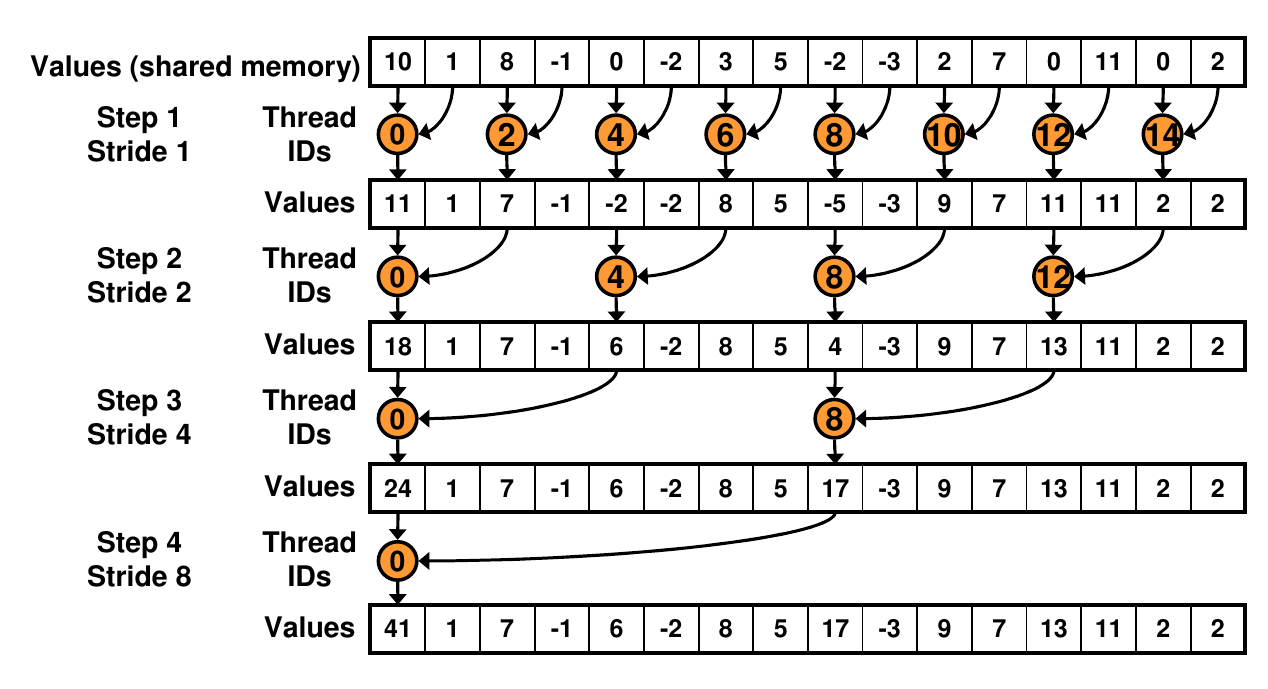
\includegraphics[scale=0.4]{1.png}		
		\end{figure}
		
		\subsection*{Schritt 2}
		Vermeiden Sie Divergenz. Indizieren Sie die Threads so, dass alle beschäftigten Threads zusammenliegen.
		
		\begin{figure}[h]
			\centering
			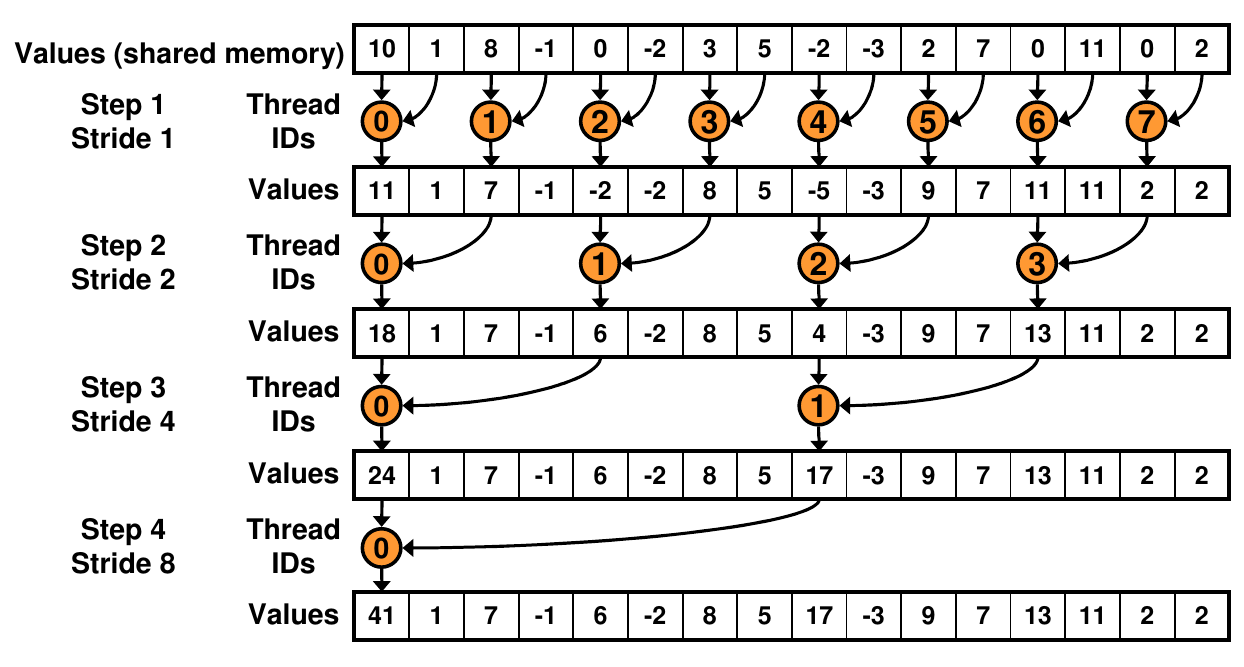
\includegraphics[scale=0.4]{2.png}		
		\end{figure}
		
		\newpage
		\subsection*{Schritt 3}
		Laden Sie die Daten in den shared Memory. Vermeiden Sie dabei Bankkonflikte. Jeder Thread muss Werte lesen, die möglichst weit auseinander liegen.
		
		\begin{figure}[h]
			\centering
			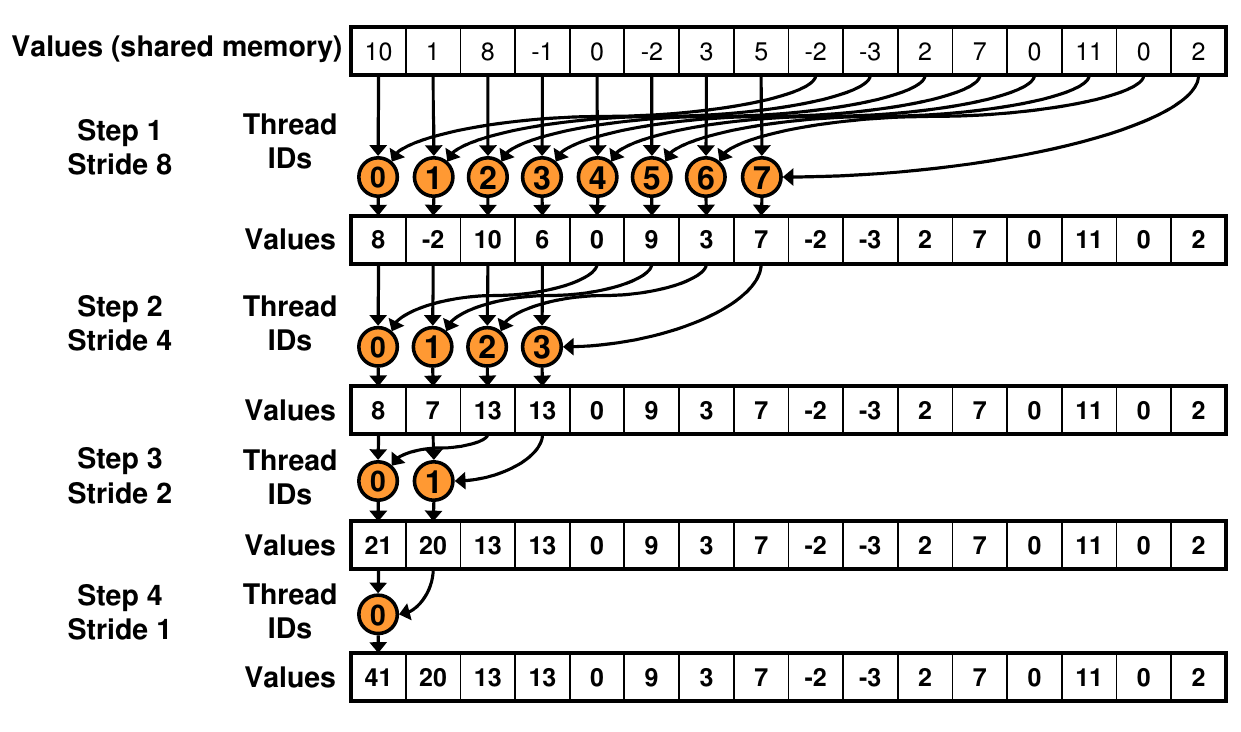
\includegraphics[scale=0.4]{3.png}		
		\end{figure}
		
		Quelle: Mark Harris: Optimizing Parallel Reduction in CUDA\\ 
		\url{https://developer.download.nvidia.com/assets/cuda/files/reduction.pdf}
		
	\section{Molekulardynamik}
	Implementieren Sie den Verlet Algorithmus\footnote{\url{https://en.wikipedia.org/wiki/Verlet_integration}}: Es befinden sich $n$ Teilchen in einem quadratischen Kasten mit Länge 1 und periodischen Randbedingungen. Jedes Teilchen wird repräsentiert durch den Ort $\vec{x}(t)$ zum Zeitpunkt $t$.
	Aus den Bewegungsgleichungen kann der Ort zu einem späteren Zeitpunkt $t+\Delta t$ berechnet werden:
	\begin{equation}
		\vec{x}(t+\Delta t) = 2\vec{x}(t) - \vec{x}(t-\Delta t) + \frac{\vec{f}}{m}\Delta t^2 + O(\Delta t^4)
	\end{equation}
	
	\begin{itemize}
		\item Vernachlässigen Sie zunächst die Kräfte.
		\item Würfeln Sie $n$ 2d Ortsektoren $\vec{x}_0$. Berechnen Sie $\vec{x}_1 = \vec{x}_0 + \vec{v}t$ mit zufälligen Geschwindigkeiten.
		\item Führen Sie parallel auf der GPU für jedes Teilchen den Iterationsschritt $\vec{x}_2 = 2\vec{x}_1 - \vec{x}_0$ aus und speichern Sie $\vec{x}_2$ zwischen.
		\item Kopieren Sie $\vec{x}_0$ nach $\vec{x}_1$ und $\vec{x}_2$ nach $\vec{x}_0$.
		\item Führen Sie das Kernel für jeden Zeitschritt aus, von $t = 0$ bis $t = t_{end}$ in Schritten von $\Delta t$.
		
		\item Berücksichtigen Sie nun die Kräfte: Die Iteration wird zu $\vec{x}_2 = 2\vec{x}_1 - \vec{x}_0 + \frac{\vec{f}_1}{m}\Delta t^2$ mit $\vec{x}_1 = \vec{x}_0 + \vec{v}t + \frac{\vec{f}_0}{m}\Delta t^2$.
		\item In jedem Schritt muss die Kraft $\vec{f}$ auf ein Teilchen $i$ berechnet werden: $\vec{f} = \sum_j \text{const}\cdot \frac{\vec{x}^i-\vec{x}^j}{|\vec{x}^i-\vec{x}^j|^3}$ ($\vec{x}^i$ bezeichnet den Ort von Teilchen $i$).
		\item Wegen der Randbedingung sollten Sie nur die Kräfte durch Teilchen innerhalb eines bestimmten Cutoff-Radius berechnen.
	\end{itemize}
	
	\section{Differentialgleichungen: Jacobi-Iteration}
	\subsection{stationäre Wärmeleitungsgleichung in zwei Dimensionen}
	Mittels Finite Difference Methoden lassen sich DGLs oft gut auf der GPU parallelisieren. Dazu versucht man Ableitungsoperatoren über einen Differenzenquotient auf einem diskreten Gitter zu nähern. Die bekanntesten Differentialgleichungen ist die Wärmeleitungsgleichung 
	\begin{equation}
		\frac{\partial}{\partial{t}}u(\vec{x,t}) - a\Laplace u(\vec{x},t) = f(\vec{x},t)
	\end{equation}
	
	mit $a > 0$ für eine Temperatur $u$ am Ort $\vec{x}$ zum Zeitpunkt $t$. Lösen Sie diese Gleichung im stationären ($\frac{\partial}{\partial{t}}u(\vec{x,t}) = 0$) und homogenen ($f(\vec{x},t) = 0$) Fall. Gleichungen dieser Gestalt bezeichnet man als Laplace-Gleichungen.
	Definieren Sie ein quadratisches Gitter ($\vec{x}=(x,y)$) und belegen Sie die Randwerte mit festen, unveränderlichen Zahlen vor (Dirichlet-Randbedingung). Wählen Sie als Gitterkonstante in beide Raumrichtungen $h_x=h_y=1$. Dann lässt sich die Laplace-Gleichung numerisch nähern als,
	\begin{equation}\label{heat}
		\Laplace u(x,y) = u(x+1,y) + u(x,y+1) + u(x-1,y) + u(x,y-1) - 4u(x,y) = 0.
	\end{equation}		 
		
	Also ist die Temperatur an jedem Ort der Mittelwert der vier Temperaturen der umgebenden Orte. Dieses Verfahren ist als \textit{five-point-stencil} bekannt.
	Schreiben Sie eine Iteration, die in jedem Schritt für jeden inneren Ort (also außer am Rand) die Temperatur neu berechnet. Dazu müssen Sie die Schleife wieder in gerade und ungerade Punkte unterteilen, um unabhängige Loops zu erhalten. Überlegen Sie sich ein vernünftiges Konvergenzkriterium und überprüfen Sie das Ergebnis, indem Sie einige Zustände in einem farbigen Plot wie in Abbildung \ref{platte} darstellen\footnote{Jeff Larkin: OpenACC Online Course 2018\\ \url{https://www.openacc.org/sites/default/files/inline-files/OpenACC_Course_Oct2018/OpenACC\%20Course\%202018\%20Week\%201.pdf}}.
	\begin{figure}[h]
		\centering
		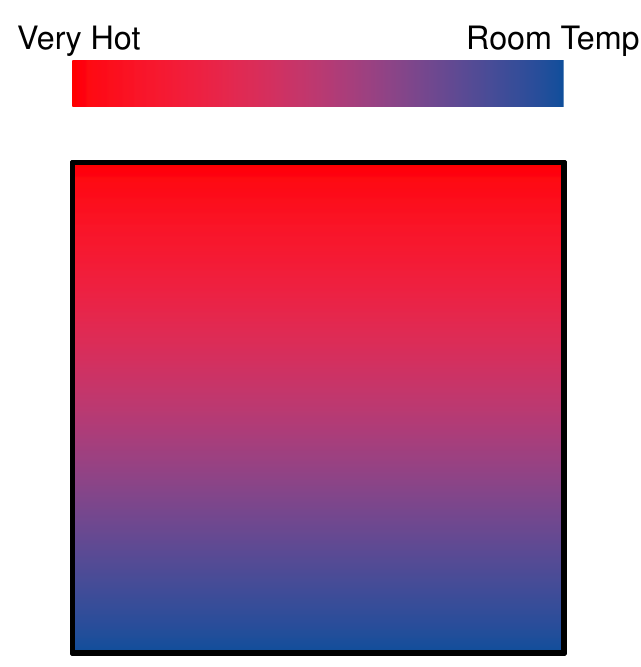
\includegraphics[scale=0.5]{platte.png}
		\caption{Wärmeleitende Platte mit konstanter Temperaturzufuhr am oberen Ende. In diesem Beispiel wurde die Gleichng (\ref{heat}) auf 50$\times$50 Punkten diskretisiert. Die Randbedingung war $u(x,0) = 1$ und $u(0,y) = u(50,y) = u(x,50) = 0$ konstant.}
		\label{platte}		
	\end{figure}
	
	\subsection{zeitabhäbgige Wärmeleitungsgleichung in einer Dimension}
	Betrachten Sie einen wärmeleitenden Stab der Länge $L$, der durch die Funktion $u(x,t)$ beschrieben wird. Dies ist die Temperatur des Stabes an Ort $0\leq x \leq L$ zum Zeitpunkt $t$. Die zu lösende homogene Differentialgleichung
	\begin{equation}\label{diff}
		\frac{\partial u}{\partial t} - \alpha\frac{\partial^2 u}{\partial x^2} = 0
	\end{equation}
	
	kann durch das Iterationsschema
	\begin{equation}\label{tps}
		u(x,t + \Delta t) = u(x,t) + \alpha \frac{\Delta t}{h^2}(u(x-h,t)-2u(x,t)+u(x+h,t))
	\end{equation}
	
	mit $h$ als Schrittweite der Diskretisierung genähert werden. Belegen Sie dazu $u(x,t=0)$ beliebig vor und setzen Sie $u(0,t)=u(L,t)=0$ als Randbedingung fest für jeden Zeitschritt. Plotten Sie die Temperaturverteilung am Anfang und am Ende, um ihr Ergebnis zu überprüfen.	
		
	\section{THRUST}
		\subsection{Saxpy}
		Schreiben Sie die \textit{Saxpy}-Operation mittels \textit{THRUST}-Funktoren, einmal mit Built-ins und einmal mit einem selbsgeschriebenen Funktor. Vergleichen Sie die Laufzeiten mit Aufgabe 2.
		
		\subsection{Varianz}
		Schreiben Sie einen Funktor zur Berechnung der Varianz eines Vektors.		
		
		\subsection{Sortieren}
		Belegen Sie einen Devicevektor zufällig mit Ganzzahlen. Sortieren Sie die erste Hälfte absteigend nach dem Rest, den man erhält, wenn man die entsprechenede Zahl durch sieben teilt, die andere Hälfte aufsteigend. 
			
			
		\section{cuRAND}
			\subsection{Pseudorandom}
			Bestimmen Sie die Kreiszahl $\pi$ durch Monte-Carlo Integration der Funktion $f(x) = \sqrt{1-x^2}$ im Bereich $[0,1]$. Würfeln Sie dazu im Quadrat $[0,1)\times[0,1)$ eine große Zahl von zweidimensionalen Punkten. Zählen Sie dabei mit, wie oft ein Punkt unterhalb der Funktion, also ob der Punkt auf der Fläche unter dem Graphen liegt. Das Verhältnis dieser Zahl zur Gesamtanzahl sollte gegen die eingeschlossene Fläche konvergieren, also gegen $\pi/4$.
			\subsection{Quasirandom}
			Bestimmen Sie die Kreiszahl $\pi$ durch Quasi-Monte-Carlo Integration. Nehmen Sie den Code aus der vorangegangenen Aufgabe und modifizieren Sie lediglich den RNG. Wahlweise lässt sich auch \textit{clQMC} verwenden. Generalisieren Sie das Programm auf $n$-dimensionale Einheitskugeln und weisen Sie nach, dass deren Volumen für $n\rightarrow\infty$ gegen 0 konvergiert.
				
		\section{Fourier Transformation}
		Vollziehen Sie für ein beliebiges komplexwertiges Eingangssignal eine 3d \textit{Complex-to-Complex} FFT in vier Versionen und vergleichen Sie die Laufzeit bei wachsender Signallänge:
		\begin{itemize}
			\item mit \textit{cuFFT} 
			\item mit \textit{clFFT}
			\item mit \textit{FFTW}
			\item mit dem \textit{FFTW} Interface für \textit{cuFFT}
		\end{itemize}	
		
		\section{BLAS}
		Vollziehen Sie in cuBLAS/clBLAS ein rank-1 update einer komplexwertigen hermiteschen $n\times n$ Matrix $A$,
		\begin{equation}
			A \leftarrow \alpha xx^H + A
		\end{equation}		 
		für  einen beliebigen Vektor $x$ und ein Skalar $\alpha$.
		
		\section{SPARSE}
		Implementieren Sie folgende Matrix mit cuSPARSE/clSPARSE:
		\begin{equation}
			A = \frac1{h^2} 
			\begin{pmatrix}
				 2      & -1      &  0     &        & \cdots &  0      \\
				-1      &  2      & -1     &  0     &        &  \vdots \\
				 0      & -1      &  2     & -1     &  0     &         \\
			    	    &  \ddots & \ddots & \ddots & \ddots &         \\
			 	 \vdots &         &  0     & -1     &  2     & -1      \\
			 	0      & \cdots  &        &  0     & -1     &  2
			\end{pmatrix}
		\end{equation}
		
		Diese Matrix entspricht einem \textit{three-point-stencil} und nähert Gleichung \ref{diff}. Die Iteration \ref{tps} lässt sich auf den inneren Gitterpunkten schreiben als $\overline{u}_{t+\Delta t} = A\overline{u}_t$ mit $\overline{u}_t = (u(h,t), u(2h,t), ... u(L-h,T))^T$\footnote{Mehr Informationen unter \url{http://www.cfd.tu-berlin.de/Lehre/tfd_skript/node46.html}}. Vergleichen Sie die Lösung dieser direkten Methode mit ihrer selbstgeschriebenen Iteration oder mit Paralution. 
		
		\section{Lineare Algebra}
		Vergleichen Sie drei Versionen einer Cholesky-Zerlegung der selben $n\times n$ Matrix $A$:
		\begin{itemize}
			\item (mit einer selbstgeschriebenen Version unter Zuhilfenahme von cuBLAS oder clBLAS)
			\item mit cuSOLVER
			\item mit MAGMA
		\end{itemize}
		$A$ muss dazu symmetrisch und positiv-definit sein. Variieren Sie $n$ und vergleichen Sie die Laufzeit. Testen Sie mit einer dünn besetzten Matrix und vergleichen Sie mit dem entsprechenden sparse-Algorithmus. 
			
%		\section{Machine Learning}
		
		\section{Projektideen}
			\subsection{Velocity-Verlet Algorithmus}
			Erweitern Sie Aufgabe 8 zum Velocity-Verlet Algorithmus. Berechnen Sie dazu explizit die Geschwindigkeiten $\vec{v}(t+\Delta t) = \vec{v}(t)+\frac{1}{2m}(\vec{f}(t)+\vec{f}(t+\Delta t))\Delta t$. Berechnen Sie in jedem Schritt die Gesamtenergie als Summe der kinetischen Energien $\frac12 m \vec{v}^2$ von jedem Teilchen. Plotten Sie diese gegen die Zeitschritte, um so die Energieerhaltung zu überprüfen und einen Langzeitdrift der Energie auszuschließen.
			
			\subsection{Ransac Algorithmus}
			Der Ransac-Algorithmus (\enquote{Random Sample Consensus}) ist ein simples Verfahren zum Fitten eines extrem verrauschten Signals. Simulieren Sie zunächst ein Signal von $s$ Messpunkten, welches einer linearen Funktion folgt. Legen Sie ein Rauschen über dieses Signal, indem Sie zusätzlich im entsprechenden Werte- und Definitionsbereich eine extrem hohe ($>>10^6$) Anzahl von uniform verteilten Punkten würfeln.
			
			Der Algorithmus versucht nun eine optimale Gerade zu finden:
			\begin{enumerate}
				\item Wählen Sie zufällig zwei Punkte aus. Diese beiden Punkte legen eine Gerade eindeutig fest.
				\item Bestimmen Sie die Anzahl an Punkten, die höchstens $\varepsilon$ von der Gerade entfernt liegen. Übersteigt diese Anzahl einen bestimmten Wert $w$, wird diese Mengen zum sogenannten Consensus Set.
				\item Wiederholen Sie die beiden Punkte beliebig oft. Das Ergebnis ist die Gerade, die den größten Konsens lieferte.
				
				\item Die resultierende Menge kann nun für einen konventionellen Fit benutzt werden.
			\end{enumerate}			 
			
			Es gibt zwei Möglichkeiten zur Parallelisierung.
			
			\begin{itemize}
				\item Parallelisieren Sie Punkt 3. Speichern Sie in jedem Schritt die Größe des Konsens. Vollziehen Sie anschließend eine Maximumsreduktion, um zu bestimmen, welche der Geraden am besten zu den Werten passt.
				\item Parallelisieren Sie Punkt 2, indem Sie die Menge aufteilen und zur Bestimmung des Konsens eine Summenreduktion vollziehen. 
			\end{itemize}			 
			
			Die Parameter $\varepsilon$ und $w$ müssen a-priori bekannt sein und vom Nutzer eingegeben werden. $\varepsilon$ sollte dabei in der Nähe der Varianz der Messwerte liegen, $w$ etwa bei deren Anzahl. Dazu muss also vorher (falls möglich) das Signal untersucht oder die Werte durch trial-and-error bestimmt werden. $w$ kann in jedem Schritt angepasst werden. Ein neuer Konsens wird nur akzeptiert, wenn dieser eine Verbesserung des alten darstellt. 
			
			Die Anzahl an benötigten Iterationen $m$ lässt sich durch Methoden der Stochastik abschätzen. Soll mit einer Wahrscheinlichkeit von $p$ mindestens einmal ein Konsens auftreten, so gilt für diese Anzahl $m = \frac{\log(1-p)}{log(1-(1-(s-w)/s)^s)}$. Besteht ein Signal zu $70\%$ aus Rauschen, so sind als nur 49 Iterationen nötig, um mit einer Wahrscheinlichkeit von $99\%$ mindestens einmal einen Konsens zu erhalten.

			\subsection{Ising Modell}
			\subsection{Replica Exchange}
			\subsection{Nullstellen komplexer Polynome}
			\subsection{G-DBSCAN}
			\subsection{Random Forest}
		
\end{document}